\documentclass{bioinfo}
\copyrightyear{2005}
\pubyear{2005}
\usepackage{graphicx}

\begin{document}
\firstpage{1}

\title[BioPax to SBML qual]{Qualitative translation of relations from BioPax to SBML qual}
\author[B\"uchel \textit{et~al}]{Finja B\"uchel\,$^{1,*}$,
and Andreas Zell\,$^1$\footnote{to whom correspondence should be addressed}}
\address{$^{1}$Department of Cognitive Systems, University of Tuebingen, Sand 1, 72076 T\"ubingen, Germany\\}


\history{Received on XXXXX; revised on XXXXX; accepted on XXXXX}

\editor{Associate Editor: XXXXXXX}

\maketitle

\begin{abstract}

\section{Motivation:}
BioPax and SBML are two of the most popular modeling languages in systems biology. The focus of SBML is the simulation and modeling of molecular pathways, whereas the BioPax specification concentrates on data exchange, visualization, and analysis of pathways. BioPax models reactions and relations. In contrast, SBML is exclusively able to handle reactions. But with the release of the SBML qual extension, it is also possible to model relations with SBML. Before this release, relations couldn't be translated to SBML or were erroneously converted to reactions. Until now, there exist no converter for BioPax to SBML, that translates reactions and relations.
\section{Results:}
Here we present the conversion of the complete nature pathway interaction database (PID) which includes pathways from BioCarta, Reactome, and from the National Cancer institute. PID provides the pathways in the BioPax Level 2 and Level 3 format. Both formats are translated to the SBML format including the qual extension. Thus, the result SBML files contain both reactions and relations.
\section{Availability:}
The complete collection of the PID models is freely available on our homepage ..... (\textbf{TODO Finja: create homepage!})
\section{Contact:} \href{finja.buechel@uni-tuebingen.de}{finja.buechel@uni-tuebingen.de}
\end{abstract}

\section{Introduction}
The goal of systems biology is the modeling and understanding of biological and chemical processes in a cell. BioPax and SBML are common modeling languages to describe such processes. The BioPax specification aims at exchanging, visualization, and analyzing such processes on a large scale. Following, BioPax can be used to image metabolic, signaling, molecular, gene regulatory and genetic interaction networks \citep{Demir2010}. In contrast, SBML is mostly used for quantitative modeling because it is well defined and homogenous \citep{Hucka2003}. The SBML core specification defines reactions in detail but no relations between molecules.
%problem
Since the release of the qual specification, it was not possible to define relations or to integrate reactions and relation in on model (\textbf{cite}).
%relevance
Furthermore, it was not possible to easily combine or exchange information between different databases, if one database uses the BioPax format and the other on the SBML format.
%literature review
So far, there exist several visualization tools, like Cytoscape, which can handle both formats (\textbf{cite}). \citet*{Ruebenacker2009} suggested a new a bridging format to solve the problem of the conversion from BioPax to SBML \citep{Ruebenacker2009}. But until now, there exists only one converter from SBML to BioPax (see http://www.ebi.ac.uk/compneur-srv/sbml/converters/SBMLtoBioPax.html) but no converter for BioPax to SBML, which's conversion also includes relations. Following, the need of combining these formats to use the knowledge different databases becomes more and more urgent.
% what we did
% necessary to mention why we use PID?
We present a complete conversion of the nature pathway interaction database (PID, \cite{Schaefer2009}) from BioPax Level 2 and Level 3 format to the SBML format including the qual extension. The pathway conversion is implemented in Java and uses jSBML and PaxTools. The translated files are freely available on our homepage: ...
% what we find out
% what do the results mean (why are they significant?)

\textbf{TODO: Clemens, Florian und Andreas: Habt ihr hier noch konkrete Ideen, was ich noch einbauen k\"onnte? Fehlt etwas?}


\begin{methods}
\section{Material and Methods}
\subsection{SBML, SBML qual, and BioPax specification}
%%%%%%%%% SBML
SBML (Systems Biology Markup Language) specification is a special XML format to describe biological models. Therefore, several classes are defined. The most important ones are species, reaction  specification defines several classes, called species, reaction \citep{Hucka2003}.
%%%%%%%%% SBML qual
\begin{itemize}
\item QualtitativeModel
\item QualitativeSpecies
\item Transition: All interactions between two or more entities, which are not molecular reactions, are named relation. These relations describe enzyme-enzyme relations, protein-protein interactions, interactions of transcription factors and genes, protein-compound interaction and links to other pathways. In SBML, qual describes relations as Transitions. Transitions consist of Input, Output, and Term objects. SBML qual specifies the kind of relation in the variable �sign� of the Input object. The sign variable can have the value �positive�, �negative�, �dual�, and �unkown�. \textbf{TODO Finja: Rewrite, because the same text in path2models}
\item Input
\item Output
\item FunctionTerm \textbf{TODO Florian: K\"onntest du hier bitte ein oder zwei S\"atze schreiben?}
\item Symbol     \textbf{TODO Florian: K\"onntest du hier bitte ein oder zwei S\"atze schreiben?}
\item
\end{itemize}

%%%%%%%%% BioPax 
BioPax Biology Pathway Exchange \citep{Demir2010}
Biopax basis=owl (Web Ontology Language)


%%%%%%%%% BioPax difference between level 2 and 3
\textbf{TODO Finja: Grobe Beschreibung, Verweis auf Publikationen}

\subsection{Conversion of BioPax to SBML qual}
%%%%%%%%% Material and implementation
\textbf{TODO: Finja rewrite, focus on PID}
 BioCarta pathways of the nature Pathway Interaction Database (PID) (2). PID provides human pathways in the BioPax format level 3 (3), which specifies for each interaction a ControlType attribute. The ControlType attribute determines if the interaction is activating or inhibiting.
Java
jSBML \citep{Draeger2011}
qual (\textbf{TODO: Citation?})
PaxTools


%%%%%%%%% Conversion
Entities 

\begin{itemize}
\item Use of Paxtools for Java einlesen
\item Use of jSBML to write the SBML qual
\item Species(Organism) is determined automatically (if it is mentioned in the file)
\item Works file vice, 1 file = 1 pathway
\item how is distinguished between a transition and a reaction... -> include table
\item annotations of the species? \textbf{TODO Clemens: K\"onntest du das bitte ausf\"uhren/erg\"anzen?SBO terms, GO,...?}
\end{itemize}


\begin{table}[!t]
\processtable{Description of the translation of BioPax control elements\label{Tab:BioPax2SBML}}
{\begin{tabular}{llll}\toprule
BioPax controller & BioPax controlled               & Converted\\
                  &                                 & SBML qual\\
                  &                                 & element\\
\midrule
\textbf{BioPax level 3}\\
\midrule
PhysicalEntity & BiochemicalReaction                & reaction\\
PhysicalEntity & ComplexAssembly                    & reaction\\
PhysicalEntity & Control                            & transition\\
PhysicalEntity & Degradation                        & transition\\
PhysicalEntity & Transport                          & transition\\
PhysicalEntity & TransportWithBiochemicalReaction   & reaction\\
PhysicalEntity & Pathway                            & transition\\
PhysicalEntity & TemplateReaction                   & transition\\
\\
Pathway         & BiochemicalReaction               & transition\\
Pathway         & ComplexAssembly                   & transition\\
Pathway         & Control                           & transition\\
Pathway         & Degradation                       & transition\\
Pathway         & Pathway                           & transition\\
Pathway         & TemplateReaction                  & transition\\
Pathway         & Transport                         & transition\\
Pathway         & TransportWithBiochemicalReaction  & transition\\
\\\midrule
\textbf{BioPax level 2}\\
\midrule
physicalEntity & biochemicalReaction                & reaction\\
physicalEntity & complexAssembly                    & reaction\\
physicalEntity & control                            & transition\\
physicalEntity & pathway                            & transition\\
physicalEntity & transport                          & transition\\
physicalEntity & transportWithBiochemicalReaction   & reaction\\
\\
pathway         & biochemicalReaction               & transition\\
pathway         & complexAssembly                   & transition\\
pathway         & control                           & transition\\
pathway         & pathway                           & transition\\
pathway         & transportWithBiochemicalReaction  & transition\\
pathway         & transport                         & transition\\\botrule
\end{tabular}}{BioPax control elements consists of a controller and one or more controlled elements. Depending on the kind of controller or controlled element, an entity is translated to a reaction or a transition. The table gives an overview of this conversion regarding BioPax level 2 and BioPax level 3.}
\end{table}



%%%%%%%%%%%%%%%%%%%%%%%%%%%%%
%% CLEMENS: MIRIAM und SBO %%
%%%%%%%%%%%%%%%%%%%%%%%%%%%%%
The BioPax specification allows users to encode arbitrary identifiers for elements. These can be identifiers for various databases, e.g., UniProt, Entrez Gene, Ensembl, etc. Unfortunately, the syntax used in BioPax is not very consistent which leads to XML elements like TODO-X or TODO-Y within BioPax documents that hamper the automatic reading and interpretation of those models by third party applications. [FINJA: BITTE DIE TODOS MIT DEM BEISPIEL <RDF UNIPROT=UNIPROT:hj35k3> und <RDF UNIPROT=hj35k3> oder \"ahnlichen uneinheitlichen beispielen f\"ullen]
In SBML, such identifiers can be expressed as standardized MIRIAM URNs that can be added as annotation to any SBML element. We support and add MIRIAM identifiers for the following databases: Entrez Gene, Omim, Ensembl, UniProt, ChEBI, DrugBank, Gene Ontology, HGNC, PubChem, 3DMET, NCBI Taxonomy, PDBeChem, GlycomeDB, LipidBank, EC-Numbers (enzyme nomeclature) and various KEGG databases (gene, glycan, reaction, compound, drug, pathway, orthology).
All supported identifiers from the BioPax files are parsed, some are manually curated (see example of inconsistent usage above) and many annotations are supplemented by additional queries to the KEGG API for every translated element. The goal of those annotations is to provide models that can be used directly by many researchers, no matter what identifiers or databases they use.

TODO: Typen (protein, gen, etc.) als SBO term in detail auflisten und erklaeren.
%%%%%%%%%%%%%%%%%%%%%%%%%%%%%


\subsection{Conversion of BioPax level 2}


\begin{figure*}[t!h]
\centering 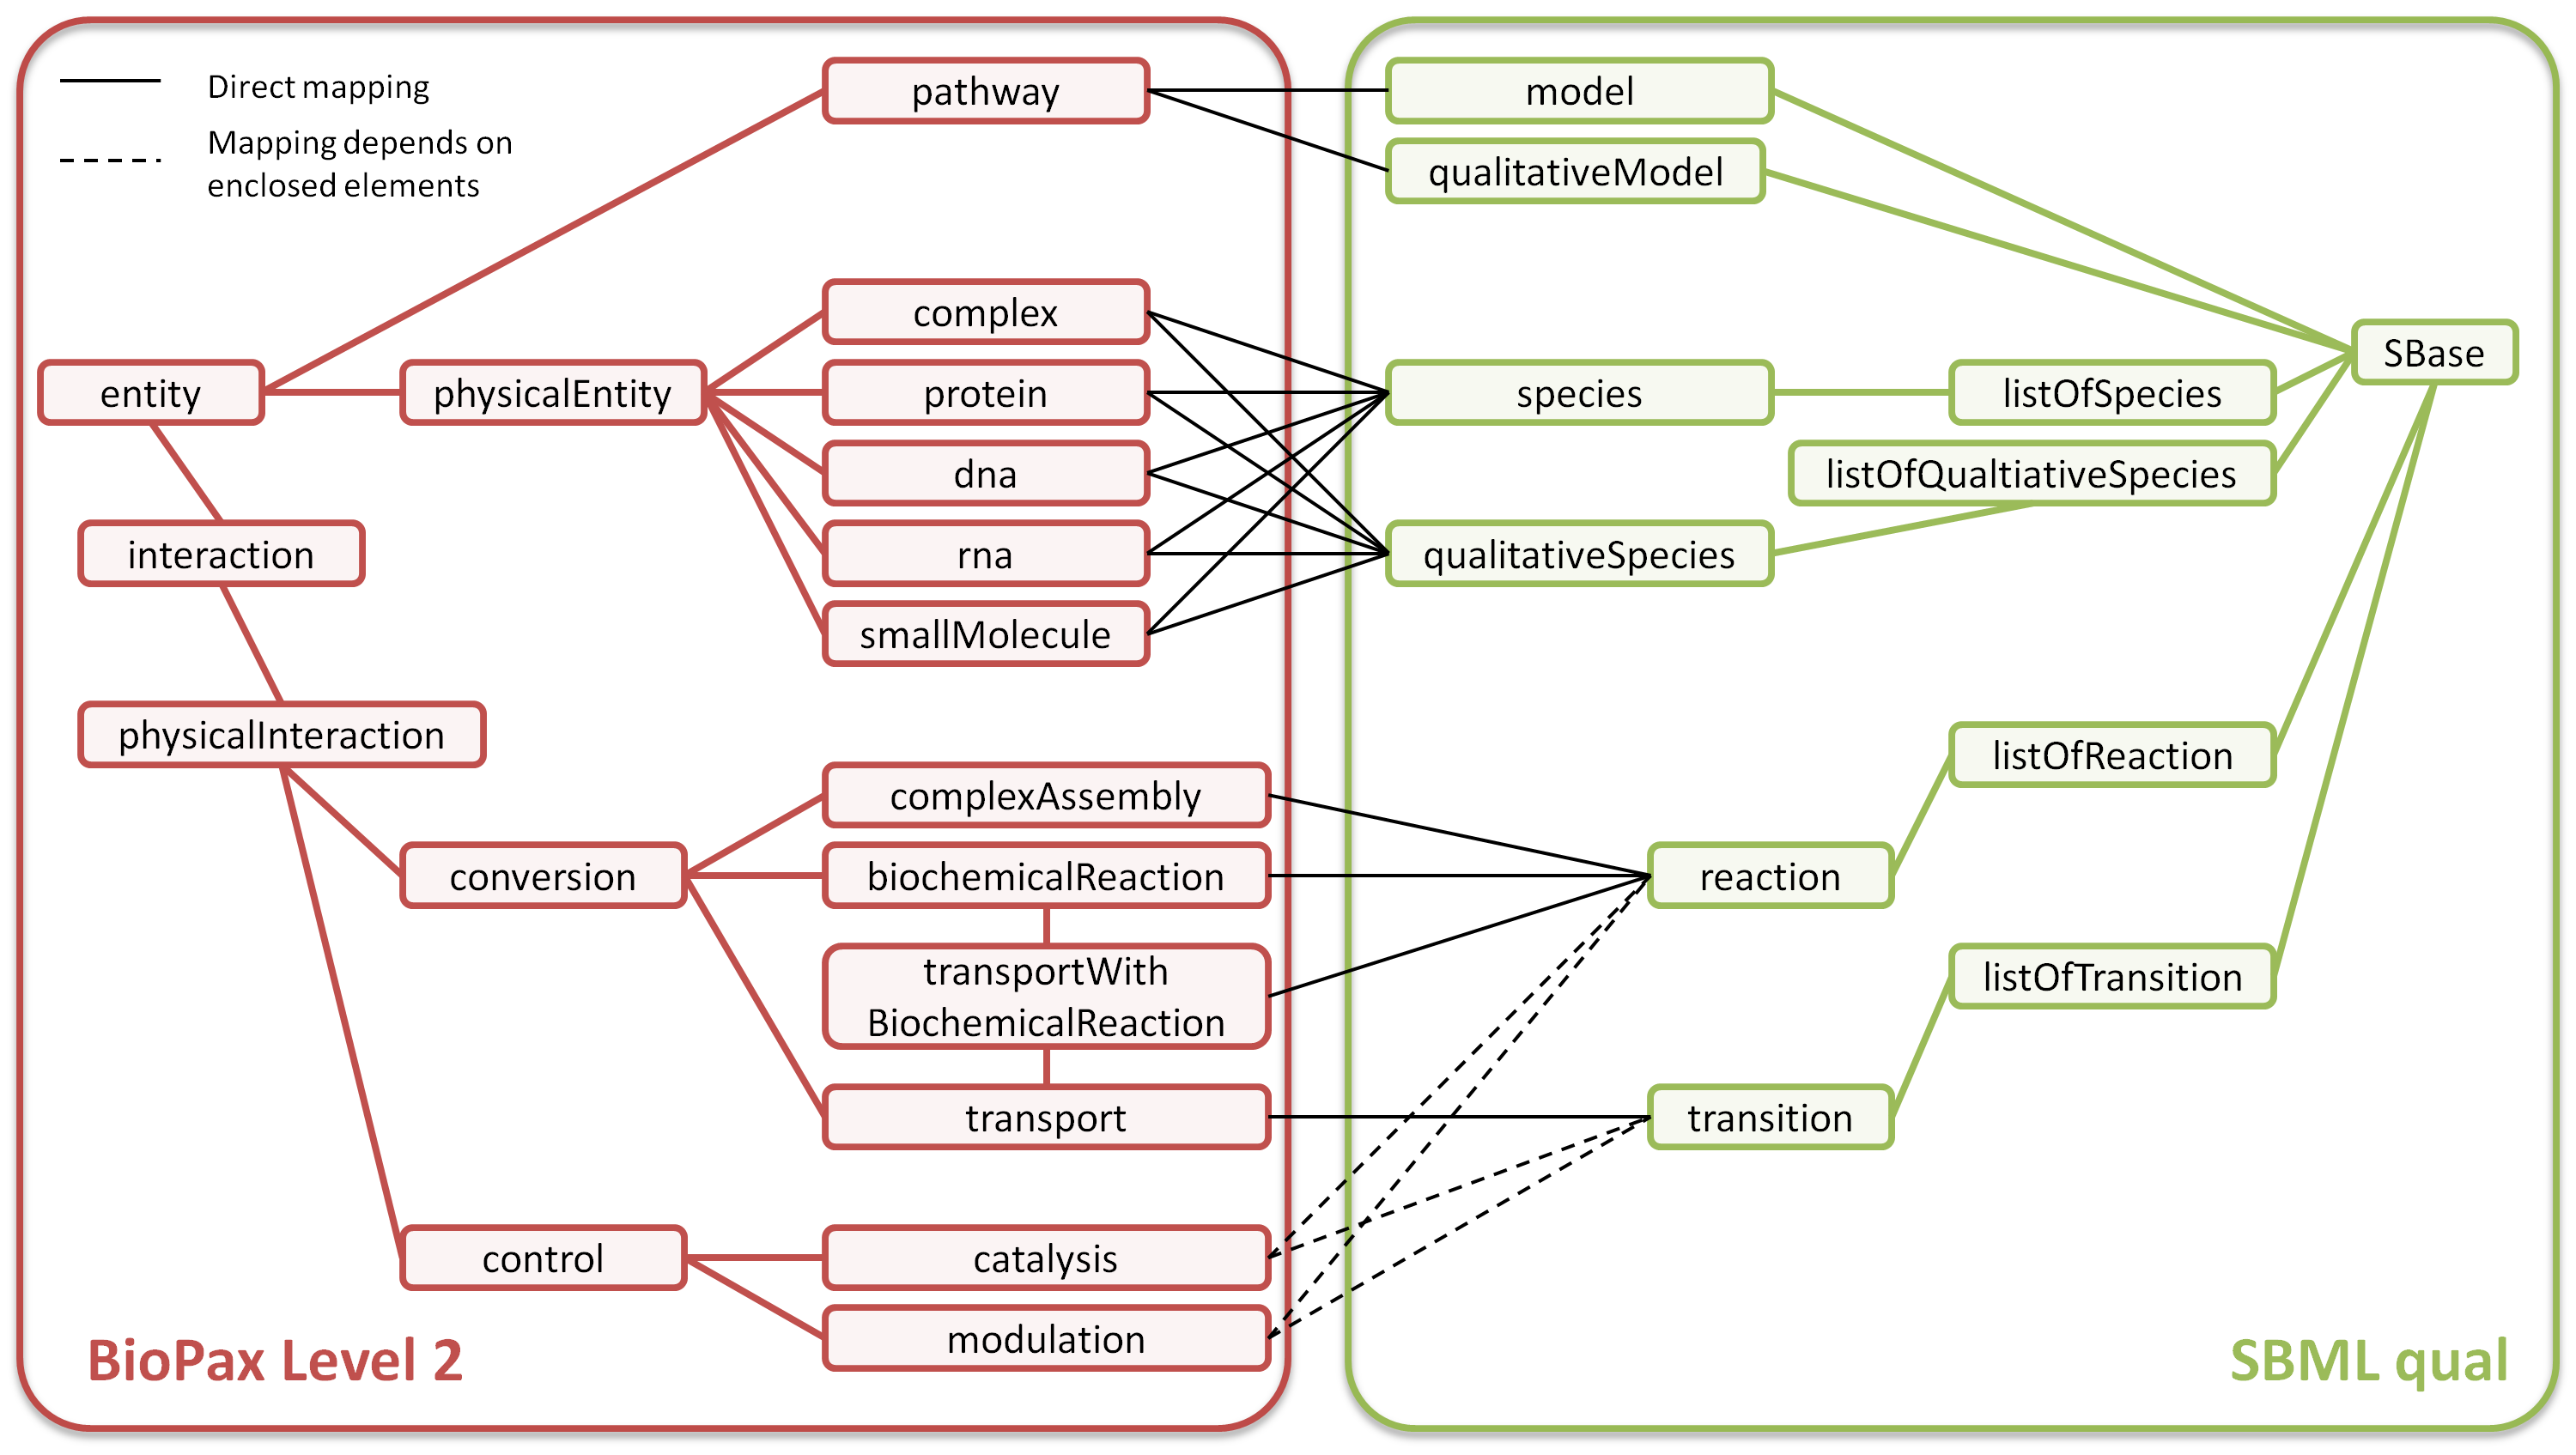
\includegraphics[width=0.96\textwidth]{BioPax2SBMLqual.png}
\caption{Conversion from BioPax Level 2 to SBML qual. The red rounded rectangles and lines describe the BioPax leve 2 elements and how they are inherited. SBML qual entities and inheritance lines are colored green. The conversion from BioPax level 2 to SBML qual is dentoted with black lines. For some elements, it depends on the enclosed element entities if BioPax is tranlsate to a reaction or a relation. These are visualized as black dashed lines. The tranlation of these elements is shown in more detail in Table \ref{Tab:BioPax2SBML}.}\label{fig:BioPax2SBMLqual}
\end{figure*}


\subsection{Conversion of BioPax level 3}
\begin{figure*}[t!h]
\centering 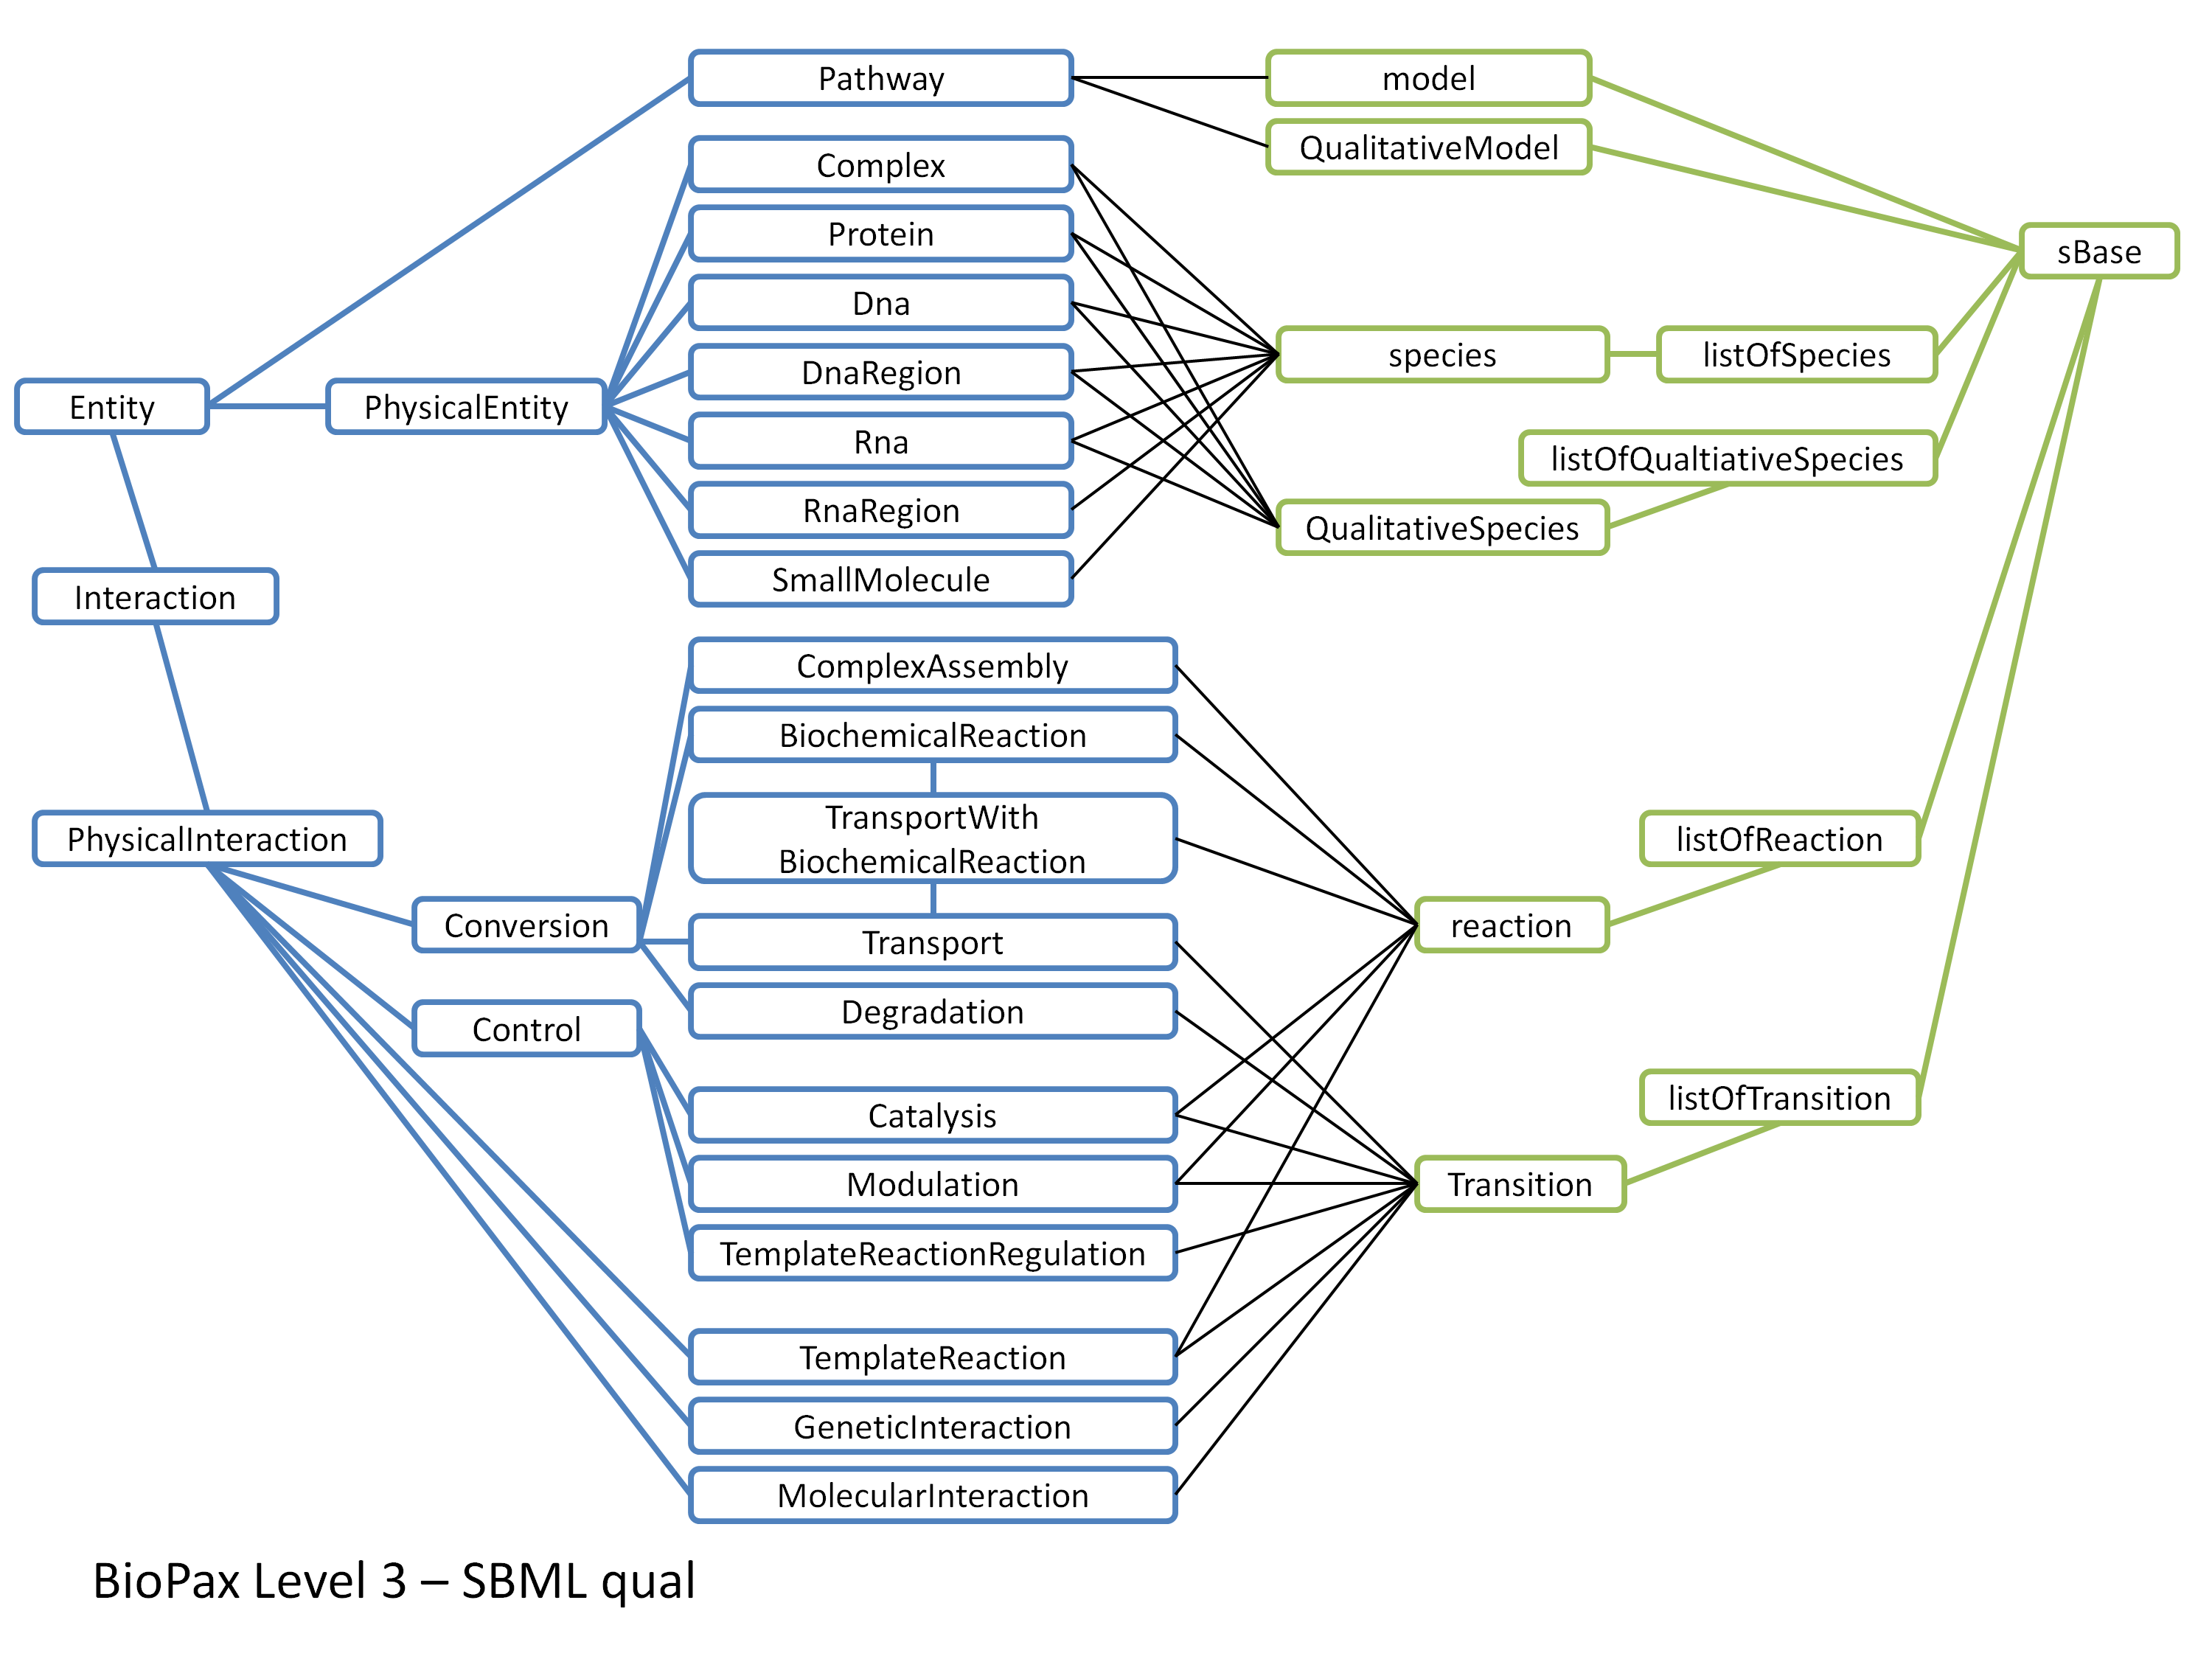
\includegraphics[width=0.96\textwidth]{BioPax3SBMLqual.png}
\caption{Conversion from BioPax Level 3 to SBML qual. The blue rounded rectangles and lines describe the BioPax leve 3 elements and how they are inherited. SBML qual entities and inheritance lines are colored green. The conversion from BioPax level 3 to SBML qual is dentoted with black lines. For some elements, it depends on the enclosed element entities if BioPax is tranlsate to a reaction or a relation. These are visualized as black dashed lines. The tranlation of these elements is shown in more detail in Table \ref{Tab:BioPax2SBML}.}\label{fig:BioPax3SBMLqual}
\end{figure*}


\begin{itemize}
\item TODO: Conversion/Control elemente nochmal zus�tzlich einzeichnen?
\item Eine example conversion einbauen?
\end{itemize}
\end{methods}


\section{Results and Discussion}
Warum ist es so toll einen converter von biopax to sbml qual zu haben?
\begin{itemize}
\item we can exchange and combine information from different databases using different model languages
\item \textbf{TODO: Clemens, Florian und Andreas: Habt ihr hier noch konkrete Erg\"anzungen?}
\end{itemize}

\section{Conclusion}

Conversions between different formats are important in all parts of computer sciences. Many conversions, in general, have errors or come with loss of information. The BioPax to SBML conversion is such an example. Due to limitations of the SBML specification, it was simply not possible to include all information from BioPax files in SBML files, while producing correct SBML code. But with SBML level 3 and the addition of extensions to the specifications, in particular the \texttt{qual} extension, it is now possible to create accurate and specification conform SBML code, and minimize or even eliminate the loss of information.

BioPax is an RDF format that defines various derived entities that can be genes, proteins, small molecules, etc. These can be translated to SBML species and the type of the entity can be encoded as SBO term or MIRIAM annotation on the species itself. Relations between entities (which correspond to edges in a pathway picture) are also provided with detailed information in BioPax. These can be transports, biochemical reactions, complex assemblies, etc. And this is the point where most conversions to SBML usually produce errors or have a massive loss of information. The SBML core specification only provides reactions, which represent real biochemical reactions with substrates, products and enzymes. But processes like the transport or modulation of an entity can not directly be encoded as a reaction, at least without knowing the exact chemical equation. Hence, former conversions from BioPax to SBML did either convert those relations to incorrect reactions or simply remove them during translation. To fill this gap, the SBML community has very recently released the \texttt{qual} specification, which allows to model arbitrary transitions between species. Using this extension, we produce error-free SBML and minimize or even eliminate the loss of information during the translation.

The SBML models provided with this publication consist of SBML-species and, wherever possible, exact reaction equations. Furthermore all relations from the BioPax documents that could not be converted to exact reactions have been included as qualitative transitions between the species. Additional information, like various identifiers or the type of an entity, are encoded as SBO terms or MIRIAM URNs of the corresponding elements. Furthermore, many information are added beyond the scope of the BioPax document by utilizing the KEGG API.

This results in comprehensive and correct SBML models, created for all pathways in the nature pathway interaction database, that can be downloaded from \href{http://TODO_INSERT_HOMEPAGE_HERE.de}{http://TODOINSERTHOMEPAGEHERE.de}. These models can easily be used, e.g., for further simulation and modeling steps, without having to deal with incorrect input file formats or error-prone conversions.

%TODO (DONE): mehr details von sbml core reations und qual relations und zusammenfassung der uebersetzung, inklusive MIRIAM annotations, sbo terms, etc. Letztendlich auf konvertierte pathways (+URL) als ultimatives ergebnis hinweisen.

\begin{itemize}
\item we provide a conversion from the most important database formats
\item we can exchange and combine information from different databases using different model languages
\item \textbf{TODO: Clemens, Florian und Andreas: Habt ihr hier noch konkrete Erg\"anzungen?}
\end{itemize}


\section*{Acknowledgement}
We thank xy.

\paragraph{Funding\textcolon} German Federal Ministry of Education and Research (BMBF) [National Genome Research Network (NGFN+) under grant number 01GS08134].

\bibliographystyle{natbib}
%\bibliographystyle{achemnat}
%\bibliographystyle{plainnat}
%\bibliographystyle{abbrv}
%\bibliographystyle{bioinformatics}
%\bibliographystyle{plain}
%
\bibliography{document}




\end{document}
